什么是用户兴趣建模呢?在很多场景中, 例如推荐、搜索、电商、广告等, 系统能够获得的数据一般是用户与系统进行交互的数据, 当然也有用户本身的一些信息, 如用户的人口特征、属性等. 我们希望对用户的兴趣/意图进行建模, 利用用户兴趣模型构建推荐/搜索系统等. 

对用户兴趣的建模也有其发展过程: 早期大多是离线计算好用户的兴趣, 大多是基于统计挖掘用户兴趣, 而后随着深度学习的发展, Deep 模型开始成为主流: 
\begin{itemize}
	\item DIN, KDD'2018; 
	\item DIEN, AAAI'2019; 
	\item MIND, CIKM'2019;
	\item DSIN, IJCAI'2019;
	\item MIMN, KDD'2019;
	\item SIM, CIKM'2020;
	\item ETA, 2021.
\end{itemize}


\subsection{基于统计的用户兴趣建模}
既然是用户的兴趣, 通常是基于用户交互过的物品来构建一些统计特征, 例如用户近期点击了哪些物品、不同类别的物品的点击次数、不同类型物品的点击率等, 或者围绕物品的一些属性进行统计, 如物品为电影时, 统计用户观看的电影中演员的分布、导演的分布等. 

\subsection{DIN}
DIN, Deep Interest Network, 诞生于阿里巴巴于 2018 年在 KDD 上发表的论文 "Deep Interest Network for Click-Through Rate Prediction". 其结构如 Fig. \ref{fig:din} 所示.

\subsubsection{Motivation}
在此之前的大部分深度 CTR 预估模型基本上遵循这样范式: 先将稀疏的输入特征 (大多是类别特征) 映射成低维的稠密向量, 然后将每个特征对应的向量聚合成定长的向量, 再将所有特征的向量进行拼接, 最后送入 MLP 中进行 CTR 的预估. 文中将这种方式描述为 Embedding\&MLP. 当以这种方式处理用户的历史行为序列时, 这类模型将用户的兴趣压缩成一个定长的向量, 不能反映出用户兴趣的多样性 --- 对于同一个用户, 其表征都是一样的. 在推荐中, 并没有必要将用户所有的兴趣压缩进一个向量, 推荐的物品只与用户的部分兴趣 (历史行为) 相关 --- 只有部分历史行为会影响当前物品的 CTR 预估. 

\subsubsection{DIN 做了什么}

\begin{figure}[h]
	\centering
	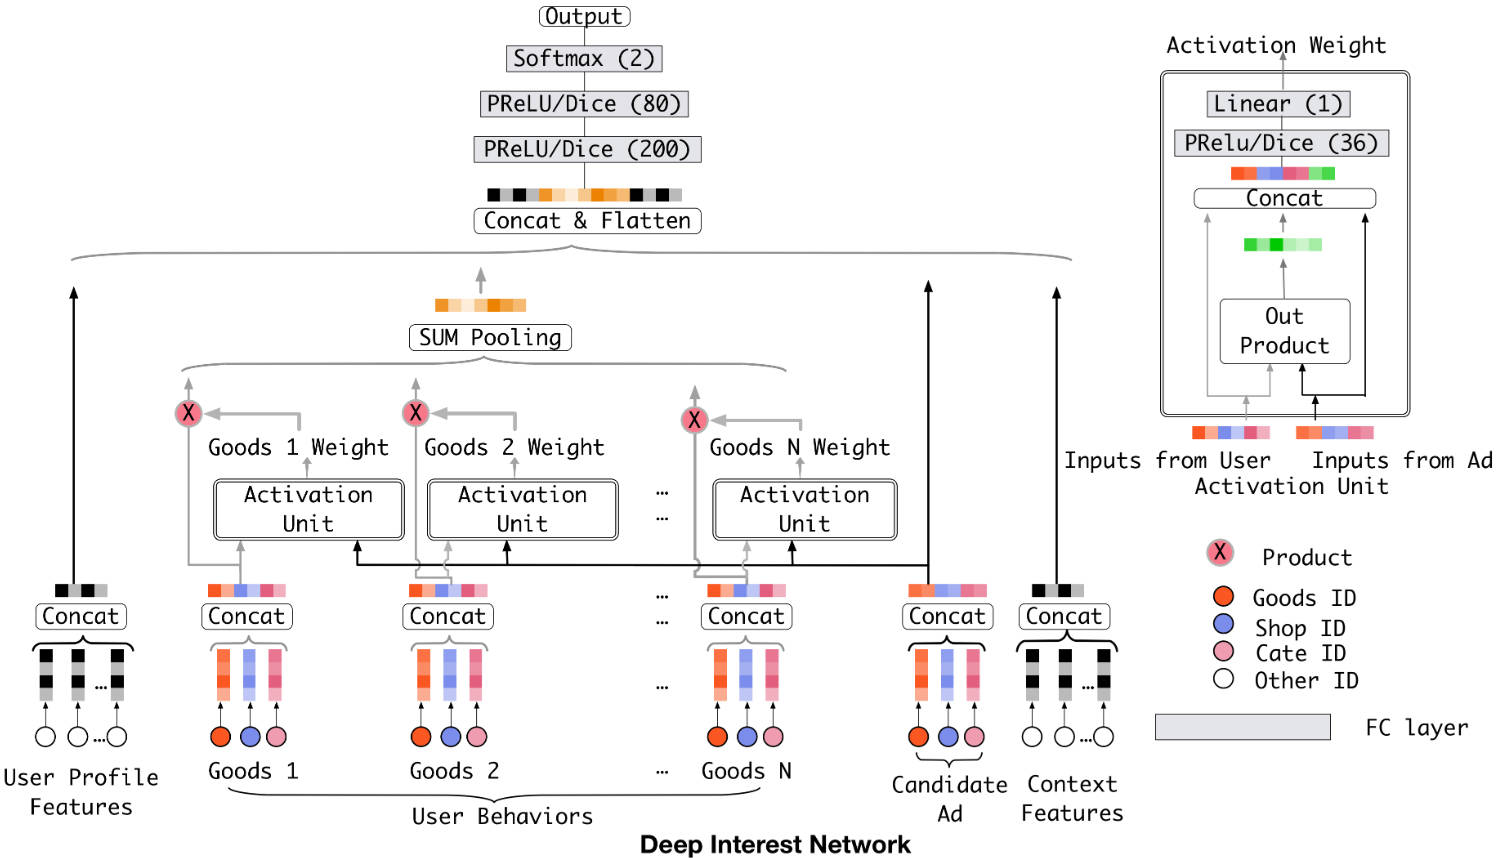
\includegraphics[width=\textwidth]{pics/din.jpg}
	\caption{Deep Interest Network}
	\label{fig:din}
\end{figure}

DIN 的主要创新体现在对用户多样化兴趣的建模上, 而这一步又是通过引入一个 Local Activation Unit 来做到的. 当然, 除此之外工程上的技术: mini-batch aware regularization、data adaptive activation function、GAUC. 其中关于用户兴趣的就是 Local Activation Unit. 

对于一个用户来说, 我们可以拿到 Ta 的行为序列, 在向其推荐物品时, 我们会有一个目标物品, 怎么利用行为序列来帮助预测呢?DIN 中利用目标物品与行为序列中物品的相关性来对用户兴趣进行建模, 即针对一个目标物品, 用户的表征/兴趣向量是其行为序列的加权求和, 权为行为序列与目标物品的相关性. 因此, 向同一个用户推荐不同的物品时, 其表征是不一样的. 相关性的计算就是通过 Local Activation Unit(LAU) 来计算的. LAU 的输入是行为序列中的物品的表征、目标物品的表征及二者的差 (论文中是 Product, 其实我感觉不重要, 只不过是前面两个的一个显式操作而已) , 三者拼接后进入前馈神经网络, 最后输出一个权重. 注意: \textbf{DIN 中并没有对这些权重进行归一化}, 论文中给出的原因是: 归一化后会弱化兴趣的强度. 

\textbf{为什么 DIN 中没有用 LSTM 来建模历史行为呢?} 论文中给出的答案是: 进行了尝试但是没有提升, 原因可能是用户行为序列与文本的不同. 文本序列是受语法约束的, 而用户的行为序列则不然, 可能同时包含多个兴趣, 可能在多个兴趣之间跳转. 

\subsubsection{不足}
\begin{myitemize}
	\item 没有考虑行为序列的序列信息, 即没有考虑物品的先后顺序. 这种情况下得到用户兴趣向量不能体现出用户的行为趋势, 而是基于整个序列进行推荐, 不是针对“下一次购买”进行推荐; 
	
	\item 只要推荐的物品与行为序列中的物品相似就会产生相似的用户向量, 即如果候选物品集都与行为序列有较高的相关性怎么办?这样产生的用户向量质量还好吗?
\end{myitemize}

\subsection{DIEN}
DIEN, Deep Interest Evolution Network, 诞生于阿里于 2019 年在 AAAI 上发表的论文 "Deep Interest Evolution Network for Click-Through Rate Prediction". 在 DIN 的基础上, DIEN 里考虑了用户兴趣的行为/兴趣的演化. 其结构如 Fig. \ref{fig:dien} 所示.

\subsubsection{Motivation}
对于 CTR 任务来说, 从用户行为背后捕捉用户的兴趣是十分关键的. 现有的一些用户兴趣建模中直接将用户行为的表示作为用户的兴趣, 而缺乏对行为背后的隐藏的兴趣的挖掘, 即行为不等价于兴趣. 并且因为外部环境和内部意识的改变, 用户的兴趣是动态的. 这些都是目前方法的不足.

\subsubsection{DIEN 怎么做的}
\begin{figure}[h]
	\centering
	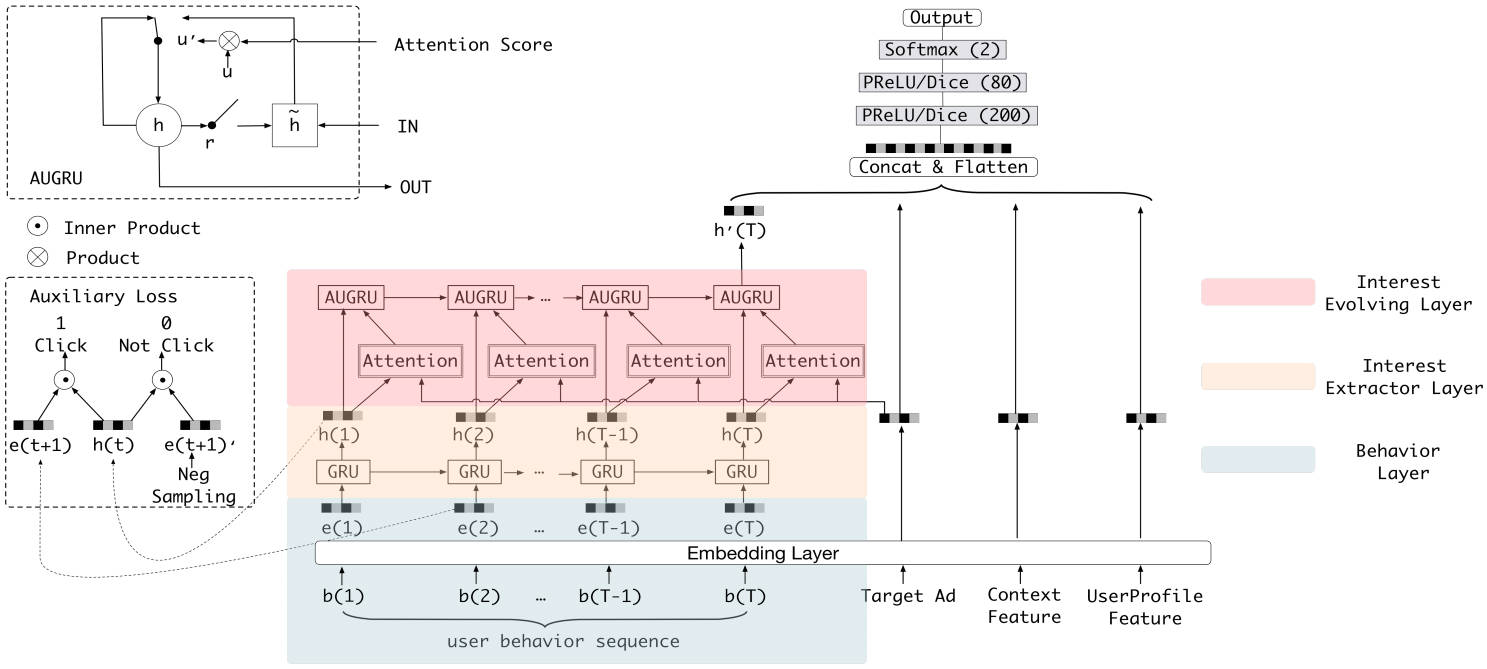
\includegraphics[width=\textwidth]{pics/dien.jpg}
	\caption{The structure of DIEN}
	\label{fig:dien}
\end{figure}

先介绍一个词, \textbf{Interest Drifting}, 兴趣漂移现象: 用户的意图在相邻的行为中可以有很大的差异, 一次行为的发生可能依赖的是很久之前的行为, 即之前的兴趣漂移到了现在, 不同的兴趣 (多峰兴趣) 有着各自的演化过程.

回顾一下 DIN: 通过嵌入层获得行为序列中每个行为的表征, 在通过局部激活单元进行 \textit{SUM Pooling}, 再与 \textit{target item} 及其他特征进行拼接, 最后输入到前馈网络中进行预测. 很明显, \textcolor{red}{DIN 直接将行为作为了用户的兴趣, 且没有考行为的序列特性}. DIEN 中通过两个模块来解决这些问题.

\paragraph{Interest Extractor Layer}
兴趣抽取层, 建模行为之间的依赖关系. DIEN 通过一个序列神经网络 (文中采用 GRU, 但就一般而言, 也可以采用其他网络, 如 LSTM, Transformer-Encoder 等) 来建模用户的连续行为, 并且引入了一个辅助损失来帮助学习来连续的行为. 这一部分的重点也就是辅助损失, 因此来看看辅助损失是怎么做的. 对于序列中的每个行为, GRU 都会输出一个 \textit{hidden state}, DIEN 中称之为 \textit{interest state}. 辅助损失将当前的行为当做 \textit{anchor}, 下一个行为作为 \textit{positive}, 随机采样一个样本作为 \textit{negative}, \textit{anchor, positive} 组成正样本, \textit{anchor, negative} 组成负样本, 以每个 \textit{anchor} 的正负样本构建损失:
$$
\begin{aligned}
	L_{a u x}=-& \frac{1}{N}\left(\sum_{i=1}^{N} \sum_{t} \log \sigma\left(\mathbf{h}_{t}^{i}, \mathbf{e}_{b}^{i}[t+1]\right)\right.\\
	&\left.+\log \left(1-\sigma\left(\mathbf{h}_{t}^{i}, \hat{\mathbf{e}}_{b}^{i}[t+1]\right)\right)\right)
\end{aligned}
$$
其中 $\mathbf{h}_t, \mathbf{e}_b^i[t+1], \hat{\mathbf{e}}_b^i[t+1]$ 分别表示 \textit{anchor, positive, negative}, $\sigma(\mathbf{x}_1, \mathbf{x}_2) = \frac{1}{1 + e^{-\mathbf{x}_1 \cdot \mathbf{x}_2}}$. 显然, $L_{aux}$ 就是个交叉熵损失函数. 引入辅助损失的好处: 1) 使 $\mathbf{h}_t$ 表达能力更强; 2) 减轻了 GRU 反向传播时的梯度弥散的问题. 

这一步, DIEN 将行为序列转换成了 \textit{interest states}, 不单单是行为序列的一个简单的表征, \textit{interest state} 还融入了序列信息, 把用户的兴趣从行为背后抽取出来.


\paragraph{Interest Evolving Layer}
兴趣演化层, \textbf{针对 \textit{target item}} 建模用户兴趣的演化过程, 其物理意义就是: 观察用户对 \textit{target item} 的兴趣在行为序列中是如何演化的. 为什么要针对 \textit{target item} 呢? 针对不同的物品 (方向), 用户的兴趣是有不同的演化路径的, 而演化路径就藏在行为序列中. 兴趣演化层可以看作是注意力机制, 把 \textit{target item} 当作 query 来匹配 key, 这一部分和 DIN 中的局部激活单元的功能是一致的. 兴趣演化层可以看作是 \textit{attention} 华和 \textit{GRU} 的结合.

首先, 是用 \textit{target item} 的表征取与兴趣抽取层每一步的输出 $\mathbf{h}_t$ 计算注意力:
$$
a_{t}=\frac{\exp \left(\mathbf{h}_{t} W \mathbf{e}_{a}\right)}{\sum_{j=1}^{T} \exp \left(\mathbf{h}_{j} W \mathbf{e}_{a}\right)}
$$
其中 $\mathbf{e}_a$ 就是 \textit{target item} 的表征. 兴趣演化层的 GRU 的输入就是兴趣抽取层的输出, 当然还把上一步计算得到的注意力融合进去, 怎么做呢? DIEN 文中设计了三种方案, 这三种方案的大体思路就是把 $a_t$ 与 GRU 里的某个部分乘起来. DIEN 中最后采用的方案是把 $a_t$ 与 GRU 中的更新门相乘, 并取名叫 \textit{GRU with attention update gate}(AUGRU). 

至此, DIEN 的结构就介绍完了.

\subsubsection{不足}
\begin{myitemize}
	\item GRU 的计算只能是串行的, 计算的时间复杂度是较高的, 在线上部署是会有较大的延迟;
\end{myitemize}


参考资料
\begin{myitemize}
	\item \href{https://mp.weixin.qq.com/s?__biz=MzU0MDA1MzI0Mw==&mid=2247488129&idx=1&sn=ed882611a06b75e8e819b519010e9e81&chksm=fb3e4915cc49c003cb4505d0b09f06fa1c4e92409270b49f5509f1902774234382ba05b400d8&scene=21#wechat_redirect}{浅谈行为序列建模};
	
	\item \href{https://mp.weixin.qq.com/s?__biz=MzI5NTU2ODQzMg==&mid=2247484150&idx=1&sn=3bdb017a542bc2e2b94404f46ec9eb4f&chksm=ec50d7a9db275ebfdc009e6be3ea6a0ee8209477dafc99bc8a6a212fa0456a14bf4453b826dd&scene=21#wechat_redirect}{刀工: 谈推荐系统特征工程中的几个高级技巧};
\end{myitemize}